% 2010 年重庆卷文科第 20 题：四棱锥 P-ABCD，底面 ABCD 为矩形，PA⊥底面，E 为棱 PB 的中点。
% 来源 PDF：普通高考/2010/2010重庆文.pdf，SHA-256 634c8ac529a6ea52305b2909eff8730888048b77d082897394bfda22cb3fe73b。
% 原页：第 2 页（A3 三栏）第 2 栏中部，书页码 580。
% 重绘依据：按原页图形比例量取顶点位置（以 BC=4 为单位长，近似）：
%   B(0,0)、C(4,0)、A(1.7,1.6)、D(5.3,1.6)、P(1.7,7.2)、E(0.85,3.6)，P 在 A 的正上方、E 为 PB 中点。
% 实线：BC、CD、PB、PC、PD、CE；虚线：PA、AB、AD、AC、AE、DE（与原页虚线段一一对应）。
% 原页在顶点 A 处画一个小叉表示该顶点被遮挡，此图照录。
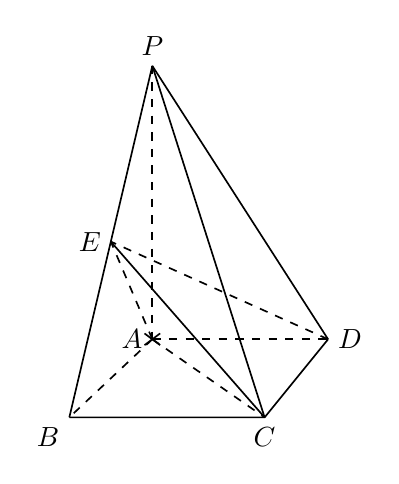
\begin{tikzpicture}[scale=0.62, semithick]
  \coordinate (B) at (0,0);
  \coordinate (C) at (4,0);
  \coordinate (A) at (1.7,1.6);
  \coordinate (D) at (5.3,1.6);
  \coordinate (P) at (1.7,7.2);
  \coordinate (E) at (0.85,3.6);

  % 可见棱
  \draw (B) -- (C) -- (D);
  \draw (P) -- (B);
  \draw (P) -- (C);
  \draw (P) -- (D);
  \draw (C) -- (E);

  % 被遮挡的棱
  \draw[dashed] (P) -- (A);
  \draw[dashed] (A) -- (B);
  \draw[dashed] (A) -- (D);
  \draw[dashed] (A) -- (C);
  \draw[dashed] (A) -- (E);
  \draw[dashed] (D) -- (E);

  % 原页在 A 处的遮挡叉号
  \draw[line width=0.6pt] (1.54,1.48) -- (1.86,1.72);
  \draw[line width=0.6pt] (1.54,1.72) -- (1.86,1.48);

  \node[above]       at (P) {$P$};
  \node[left]        at (E) {$E$};
  \node[left]        at (A) {$A$};
  \node[below left]  at (B) {$B$};
  \node[below]       at (C) {$C$};
  \node[right]       at (D) {$D$};
\end{tikzpicture}
